\begin{figure}[ht]
\centering
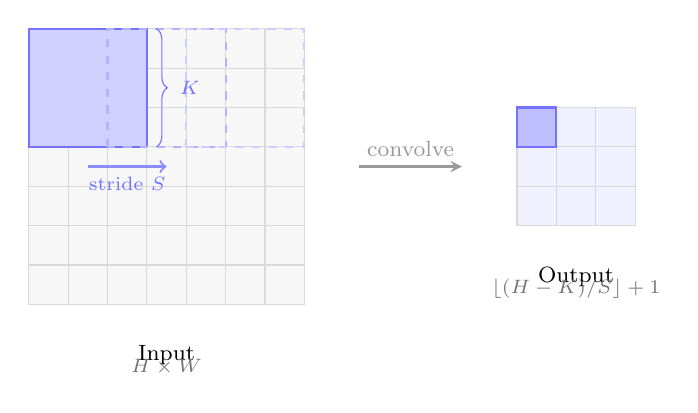
\begin{tikzpicture}[
    arr/.style={->, thick, >=stealth, black!40},
    lbl/.style={font=\footnotesize},
    sublbl/.style={font=\scriptsize, text=black!55}
]

\def\c{0.5}

% --- Input grid (7x7) ---
\foreach \x in {0,...,6} {
    \foreach \y in {0,...,6} {
        \fill[gray!6, draw=black!15]
            (\x*\c, \y*\c) rectangle ({(\x+1)*\c}, {(\y+1)*\c});
    }
}

% Kernel position 1 (solid)
\fill[blue!18, draw=blue!55, thick]
    (0, {4*\c}) rectangle ({3*\c}, {7*\c});

% Kernel position 2 (dashed, shifted by stride 2)
\draw[blue!30, thick, dashed]
    ({2*\c}, {4*\c}) rectangle ({5*\c}, {7*\c});

% Kernel position 3 (dashed, shifted again)
\draw[blue!20, thick, dashed]
    ({4*\c}, {4*\c}) rectangle ({7*\c}, {7*\c});

% Stride arrow
\draw[->, thick, blue!45]
    ({1.5*\c}, {3.5*\c}) -- ({3.5*\c}, {3.5*\c})
    node[midway, below, font=\scriptsize, blue!55] {stride $S$};

% Kernel size brace (right side of kernel)
\draw[decorate, decoration={brace, amplitude=4pt}, blue!55]
    ({3*\c + 0.12}, {7*\c}) -- ({3*\c + 0.12}, {4*\c})
    node[midway, right=5pt, font=\scriptsize, blue!55] {$K$};

% Input label
\node[lbl, anchor=north] at ({3.5*\c}, -0.4) {Input};
\node[sublbl] at ({3.5*\c}, -0.8) {$H \times W$};

% Arrow
\draw[arr] ({7*\c + 0.7}, {3.5*\c}) -- ({7*\c + 2.0}, {3.5*\c})
    node[midway, above, lbl] {convolve};

% --- Output grid (3x3) ---
\def\ox{6.2}
\foreach \x in {0,...,2} {
    \foreach \y in {0,...,2} {
        \fill[blue!6, draw=black!15]
            ({\ox + \x*\c}, {2*\c + \y*\c})
            rectangle ({\ox + (\x+1)*\c}, {2*\c + (\y+1)*\c});
    }
}

% Highlighted output cell (corresponds to kernel pos 1)
\fill[blue!25, draw=blue!55, thick]
    (\ox, {4*\c}) rectangle ({\ox + \c}, {5*\c});

% Output label
\node[lbl, anchor=north] at ({\ox + 1.5*\c}, {2*\c - 0.4}) {Output};
\node[sublbl] at ({\ox + 1.5*\c}, {2*\c - 0.8})
    {$\lfloor(H - K) / S\rfloor + 1$};

\end{tikzpicture}
\caption{Convolution operation. A $K \times K$ kernel slides across
  the input with stride $S$. Each position produces one output value.
  Dashed outlines show subsequent kernel positions.}
\label{fig:conv-operation}
\end{figure}
